%  LaTeX support: latex@mdpi.com 
%  For support, please attach all files needed for compiling as well as the log file, and specify your operating system, LaTeX version, and LaTeX editor.

%=================================================================
\documentclass[journal,article,submit,pdftex,moreauthors]{Definitions/mdpi} 
%\documentclass[preprints,article,submit,pdftex,moreauthors]{Definitions/mdpi} 
% For posting an early version of this manuscript as a preprint, you may use "preprints" as the journal. Changing "submit" to "accept" before posting will remove line numbers.

% Below journals will use APA reference format:
% admsci, aieduc, behavsci, businesses, econometrics, economies, education, ejihpe, famsci, games, humans, ijcs, ijfs, jintelligence, journalmedia, jrfm, jsam, languages, peacestud, psycholint, publications, tourismhosp, youth

% Below journals will use Chicago reference format:
% arts, genealogy, histories, humanities, laws, literature, religions, risks, socsci

%--------------------
% Class Options:
%--------------------
%----------
% journal
%----------
% Choose between the following MDPI journals:
% accountaudit, acoustics, actuators, addictions, adhesives, admsci, adolescents, aerobiology, aerospace, agriculture, agriengineering, agrochemicals, agronomy, ai, aichem, aieduc, aieng, aimater, aimed, aipa, air, aisens, algorithms, allergies, alloys, amh, analog, analytica, analytics, anatomia, anesthres, animals, antibiotics, antibodies, antioxidants, applbiosci, appliedchem, appliedmath, appliedphys, applmech, applmicrobiol, applnano, applsci, aquacj, architecture, arm, arthropoda, arts, asc, asi, astronautics, astronomy, atmosphere, atoms, audiolres, automation, axioms, bacteria, batteries, bdcc, behavsci, beverages, biochem, bioengineering, biologics, biology, biomass, biomechanics, biomed, biomedicines, biomedinformatics, biomimetics, biomolecules, biophysica, bioresourbioprod, biosensors, biosphere, biotech, birds, blockchains, bloods, blsf, brainsci, breath, buildings, businesses, cancers, carbon, cardio, cardiogenetics, cardiovascmed, catalysts, cells, ceramics, challenges, chemengineering, chemistry, chemosensors, chemproc, children, chips, cimb, civileng, cleantechnol, climate, clinbioenerg, clinpract, clockssleep, cmd, cmtr, coasts, coatings, colloids, colorants, commodities, complexities, complications, compounds, computation, computers, condensedmatter, conservation, constrmater, cosmetics, covid, crops, cryo, cryptography, crystals, csmf, ctn, culture, curroncol, cyber, dairy, data, ddc, dentistry, dermato, dermatopathology, designs, devices, dhi, diabetology, diagnostics, dietetics, digital, disabilities, diseases, diversity, dna, drones, dynamics, earth, ebj, ecm, ecologies, econometrics, economies, edm, education, eesp, ejihpe, electricity, electrochem, electronicmat, electronics, encyclopedia, endocrines, energies, eng, engproc, entomology, entropy, environments, environremediat, epidemiologia, epigenomes, esa, est, famsci, fermentation, fibers, fintech, fire, fishes, fluids, foods, forecasting, forensicsci, forests, fossstud, foundations, fractalfract, fuels, future, futureinternet, futurepharmacol, futurephys, futuretransp, galaxies, games, gases, gastroent, gastrointestdisord, gastronomy, gels, genealogy, genes, geographies, geohazards, geomatics, geometry, geosciences, geotechnics, geriatrics, germs, glacies, grasses, green, greenhealth, gucdd, hardware, hazardousmatters, healthcare, hearts, hemato, hematolrep, hep, heritage, higheredu, highthroughput, histories, horticulturae, hospitals, humanities, humans, hydrobiology, hydrogen, hydrology, hydropower, hygiene, idr, iic, ijcs, ijem, ijerph, ijfs, ijgi, ijmd, ijms, ijns, ijom, ijpb, ijt, ijtm, ijtpp, ime, immuno, informatics, information, infrastructures, inorganics, insects, instruments, inventions, iot, j, jaestheticmed, jal, jcdd, jcm, jcp, jcrm, jcs, jcto, jdad, jdb, jdream, jemr, jeta, jfb, jfmk, jgbg, jgg, jimaging, jintelligence, jlpea, jmahp, jmmp, jmms, jmp, jmse, jne, jnt, jof, joi, joitmc, joma, jop, joptm, jor, journalmedia, jox, jpbi, jphytomed, jpm, jrfm, jsam, jsan, jtaer, jvd, jzbg, kidneydial, kinasesphosphatases, knowledge, labmed, laboratories, lae, land, languages, laws, life, lights, limnolrev, lipidology, liquids, literature, livers, logics, logistics, lubricants, lymphatics, machines, macromol, magnetism, magnetochemistry, make, marinedrugs, materials, materproc, mathematics, mca, measurements, medicina, medicines, medsci, membranes, merits, metabolites, metals, meteorology, methane, metrics, metrology, micro, microarrays, microbiolres, microelectronics, micromachines, microorganisms, microplastics, microwave, minerals, mining, mmphys, modelling, molbank, molecules, mps, msf, mti, multimedia, muscles, nanoenergyadv, nanomanufacturing, nanomaterials, ncrna, ndt, network, neuroglia, neuroimaging, neurolint, neurosci, nitrogen, notspecified, nursrep, nutraceuticals, nutrients, obesities, occuphealth, oceans, ohbm, onco, optics, oral, organics, organoids, osteology, oxygen, pandemics, parasites, parasitologia, particles, pathogens, pathophysiology, peacestud, pediatrrep, pets, pharmaceuticals, pharmaceutics, pharmacoepidemiology, pharmacy, philosophies, photochem, photonics, phycology, physchem, physics, physiologia, plants, plasma, platforms, pollutants, polymers, polysaccharides, populations, poultry, powders, precipitation, precisoncol, preprints, proceedings, processes, prosthesis, proteomes, psf, psychiatryint, psychoactives, psycholint, publications, purification, quantumrep, quaternary, qubs, radiation, rdt, reactions, realestate, receptors, recycling, regeneration, religions, remotesensing, reports, reprodmed, resources, rheumato, risks, rjpm, robotics, rsee, ruminants, safety, sci, scipharm, sclerosis, seeds, sensors, separations, sexes, shi, signals, sinusitis, siuj, skins, smartcities, sna, societies, socsci, software, soilsystems, solar, solids, spectroscj, sports, standards, stats, std, stratsediment, stresses, surfaces, surgeries, suschem, sustainability, symmetry, synbio, systems, tae, targets, taxonomy, technologies, telecom, test, textiles, thalassrep, therapeutics, thermo, timespace, tomography, tourismhosp, toxics, toxins, tph, transplantology, transportation, traumacare, traumas, tri, tropicalmed, universe, urbansci, uro, vaccines, vehicles, venereology, vetsci, vibration, virtualworlds, viruses, vision, waste, water, welding, wem, wevj, wild, wind, women, world, youth, zoonoticdis

%---------
% article
%---------
% The default type of manuscript is "article", but can be replaced by: 
% abstract, addendum, article, benchmark, book, bookreview, briefcommunication, briefreport, casereport, changes, clinicopathologicalchallenge, comment, commentary, communication, conceptpaper, conferenceproceedings, correction, conferencereport, creative, datadescriptor, discussion, entry, expressionofconcern, extendedabstract, editorial, essay, erratum, fieldguide, hypothesis, interestingimages, letter, meetingreport, monograph, newbookreceived, obituary, opinion, proceedingpaper, projectreport, reply, retraction, review, perspective, protocol, shortnote, studyprotocol, supfile, systematicreview, technicalnote, viewpoint, guidelines, registeredreport, tutorial,  giantsinurology, urologyaroundtheworld
% supfile = supplementary materials

%----------
% submit
%----------
% The class option "submit" will be changed to "accept" by the Editorial Office when the paper is accepted. This will only make changes to the frontpage (e.g., the logo of the journal will get visible), the headings, and the copyright information. Also, line numbering will be removed. Journal info and pagination for accepted papers will also be assigned by the Editorial Office.

%------------------
% moreauthors
%------------------
% If there is only one author the class option oneauthor should be used. Otherwise use the class option moreauthors.

%---------
% pdftex
%---------
% The option pdftex is for use with pdfLaTeX. Remove "pdftex" for (1) compiling with LaTeX & dvi2pdf (if eps figures are used) or for (2) compiling with XeLaTeX.

%=================================================================
% MDPI internal commands - do not modify
\firstpage{1} 
\makeatletter 
\setcounter{page}{\@firstpage} 
\makeatother
\pubvolume{1}
\issuenum{1}
\articlenumber{0}
\pubyear{2026}
\copyrightyear{2026}
%\externaleditor{Firstname Lastname} % More than 1 editor, please add `` and '' before the last editor name
\datereceived{ } 
\daterevised{ } % Comment out if no revised date
\dateaccepted{ } 
\datepublished{ } 
%\datecorrected{} % For corrected papers: "Corrected: XXX" date in the original paper.
%\dateretracted{} % For retracted papers: "Retracted: XXX" date in the original paper.
%\doinum{} % Used for some special journals, like molbank
%\pdfoutput=1 % Uncommented for upload to arXiv.org
%\CorrStatement{yes}  % For updates
%\longauthorlist{yes} % For many authors that exceed the left citation part
%\IsAssociation{yes} % For association journals

%=================================================================
% Add packages and commands here. The following packages are loaded in our class file: fontenc, inputenc, calc, indentfirst, fancyhdr, graphicx, epstopdf, lastpage, ifthen, float, amsmath, amssymb, lineno, setspace, enumitem, mathpazo, booktabs, titlesec, etoolbox, tabto, xcolor, colortbl, soul, multirow, microtype, tikz, totcount, changepage, attrib, upgreek, array, tabularx, pbox, ragged2e, tocloft, marginnote, marginfix, enotez, amsthm, natbib, hyperref, cleveref, scrextend, url, geometry, newfloat, caption, draftwatermark, seqsplit
% cleveref: load \crefname definitions after \begin{document}

%=================================================================
% Please use the following mathematics environments: Theorem, Lemma, Corollary, Proposition, Characterization, Property, Problem, Example, ExamplesandDefinitions, Hypothesis, Remark, Definition, Notation, Assumption
%% For proofs, please use the proof environment (the amsthm package is loaded by the MDPI class).

%=================================================================
% Full title of the paper (Capitalized)
\Title{Evaluating Parameter-Efficient Fine-Tuning vs. Prompt Engineering for Profile-Driven Recommendations}

% Author Orchid ID: enter ID or remove command
\newcommand{\orcidauthorA}{0009-0002-1965-7822}%LS
\newcommand{\orcidauthorB}{0009-0004-4210-5756}%RK
\newcommand{\orcidauthorC}{0000-0002-3015-1024}%SBS
\newcommand{\orcidauthorE}{0000-0002-5964-245X}%IL
%\newcommand{\orcidauthorB}{0000-0000-0000-000X} % Add \orcidB{} behind the author's name

% Authors, for the paper (add full first names)
\Author{Luka Sever $^{1}$\orcidA{}, Ratomir Karlović $^{1}$\orcidB{}, Sandi Baressi Šegota $^{1}$\orcidC{} and Ivan Lorencin $^{1}$\orcidE{}}

%\longauthorlist{yes}

% MDPI internal command: Authors, for metadata in PDF
\AuthorNames{Luka Sever, Ratomir Karlović, Sandi Baressi Šegota and Ivan Lorencin}

%\longauthorlist{yes}

% Affiliations / Addresses (Add [1] after \address if there is only one affiliation.)
\address{%
$^{1}$ \quad Faculty of Informatics, Juraj Dobrila University of Pula, Zagrebačka 30, 52100 Pula, Croatia;\\ luka.sever@unipu.hr (L.S.), ratomir.karlovic@unipu.hr (R.K.), sandi.baressi.segota@unipu.hr (S.B.Š.), ivan.lorencin@unipu.hr (I.L.)\\
% $^{2}$ \quad Affiliation 2; e-mail@e-mail.com
}

% Contact information of the corresponding author
\corres{Correspondence: sandi.baressi.segota@unipu.hr}

% Current address and/or shared authorship
%\firstnote{Current address: Affiliation.}  
% Current address should not be the same as any items in the Affiliation section.

%\secondnote{These authors contributed equally to this work.}
% The commands \thirdnote{} till \eighthnote{} are available for further notes.

%\simplesumm{} % Simple summary

%\conference{} % An extended version of a conference paper

% Abstract (Do not insert blank lines, i.e. \\) 
\abstract{Large language models (LLMs) show significant promise for personalized recommendation systems, yet identifying the most effective adaptation strategy for structured data remains a challenge. This study compares parameter-efficient fine-tuning (PEFT) and in-context learning approaches for personalized item recommendation. We utilized explicit user profiles, encompassing specific likes and dislikes, alongside a comprehensive JSON-formatted item catalog. Two distinct adaptation paradigms were compared on Llama 3.1 8B and Llama 3.2 3B: PEFT, specifically Low-Rank Adaptation (LoRA) and Infused Adapter by Inhibiting and Amplifying Inner Activations (IA$^3$), against prompt engineering strategies optimizing input instructions without altering model weights. Because personalized recommendation is inherently subjective and has no objective ground truth, three human annotators independently judged 1,521 recommendations per configuration as agreeing (1), disagreeing ($-1$) or neither (0) with the recommendation, and the consistency of their judgments was quantified using Fleiss' kappa ($\kappa$). Agreement was almost perfect in all six configurations ($\kappa$ between 0.863 and 0.904), indicating a reliable evaluation protocol. Fine-tuned adapters yielded higher agreement than the prompt-engineered baseline for both foundation models, although the differences between configurations were small (at most 0.041), only one of them (LoRA on Llama 3.1 8B) remained statistically significant after correction for multiple comparisons, and no single adapter type was consistently superior across models. These results show that adapter-based fine-tuning produces recommendations whose relevance to explicit user profiles is judged at least as consistently as that of prompt engineering alone.}

% Keywords
\keyword{large language models; parameter-efficient fine-tuning; prompt engineering; recommender systems; Low-Rank Adaptation (LoRA); structured data processing; in-context learning}

% The fields PACS, MSC, and JEL may be left empty or commented out if not applicable
%\PACS{J0101}
%\MSC{}
%\JEL{}

%%%%%%%%%%%%%%%%%%%%%%%%%%%%%%%%%%%%%%%%%%
% Only for the journal Diversity
%\LSID{\url{http://}}

%%%%%%%%%%%%%%%%%%%%%%%%%%%%%%%%%%%%%%%%%%
% Only for the journal Applied Sciences
%\featuredapplication{Authors are encouraged to provide a concise description of the specific application or a potential application of the work. This section is not mandatory.}
%%%%%%%%%%%%%%%%%%%%%%%%%%%%%%%%%%%%%%%%%%

%%%%%%%%%%%%%%%%%%%%%%%%%%%%%%%%%%%%%%%%%%
% Only for the journal Data
%\dataset{DOI number or link to the deposited data set if the data set is published separately. If the data set shall be published as a supplement to this paper, this field will be filled by the journal editors. In this case, please submit the data set as a supplement.}
%\datasetlicense{License under which the data set is made available (CC0, CC-BY, CC-BY-SA, CC-BY-NC, etc.)}

%%%%%%%%%%%%%%%%%%%%%%%%%%%%%%%%%%%%%%%%%%
% Only for the journal BioTech, Fishes, Neuroimaging and Toxins
%\keycontribution{The breakthroughs or highlights of the manuscript. Authors can write one or two sentences to describe the most important part of the paper.}

%%%%%%%%%%%%%%%%%%%%%%%%%%%%%%%%%%%%%%%%%%
% Only for the journal Encyclopedia
%\encyclopediadef{For entry manuscripts only: please provide a brief overview of the entry title instead of an abstract.}

%%%%%%%%%%%%%%%%%%%%%%%%%%%%%%%%%%%%%%%%%%
% Different journals have different requirements. Please check the specific journal guidelines in the "Instructions for Authors" on the journal's official website.
%\addhighlights{yes}
%\renewcommand{\addhighlights}{%
%
%\noindent The goal is to increase the discoverability and readability of the article via search engines and other scholars. Highlights should not be a copy of the abstract, but a simple text allowing the reader to quickly and simplified find out what the article is about and what can be cited from it. Each of these parts should be devoted up to 2~bullet points.\vspace{3pt}\\
%\textbf{What are the main findings?}
% \begin{itemize}[labelsep=2.5mm,topsep=-3pt]
% \item First bullet.
% \item Second bullet.
% \end{itemize}\vspace{3pt}
%\textbf{What are the implications of the main findings?}
% \begin{itemize}[labelsep=2.5mm,topsep=-3pt]
% \item First bullet.
% \item Second bullet.
% \end{itemize}
%}

%%%%%%%%%%%%%%%%%%%%%%%%%%%%%%%%%%%%%%%%%%
\begin{document}

%%%%%%%%%%%%%%%%%%%%%%%%%%%%%%%%%%%%%%%%%%

\section{Introduction}

The integration of Large Language Models (LLMs) into recommendation systems has fundamentally transformed the field, treating recommendation as a sequence generation task. However, adapting these models to dynamic user preferences presents significant challenges regarding stability and plasticity. To address the continuous evolution of users and items, recent research has explored parameter-efficient fine-tuning (PEFT) methods like Low-Rank Adaptation (LoRA); for instance, the PESO framework maintains a single evolving adapter anchored by a proximal term to dynamically capture new user behaviors while mitigating the catastrophic forgetting associated with sequential updates \citep{yoo2025continual}. 

Transitioning LLMs into conversational recommenders introduces additional complexities, particularly concerning semantic misalignment and cumbersome training processes. To streamline this, the PECRS framework reformulates the problem entirely as a natural language processing task, utilizing a frozen pre-trained language model and rich textual metadata to perform both item recommendation and response generation. This unified architecture can be optimized in a single training stage using PEFT techniques, significantly reducing computational overhead \citep{ravaut2024parameter}. 

While efficiency is crucial, standard PEFT methods often lack parameter-level personalization because they rely on a static, shared LoRA module for all users. The RecLoRA framework addresses this by introducing a Personalized LoRA module, which dynamically generates unique weights for each user through a soft routing mechanism guided by a conventional recommendation model \citep{zhu2024lifelong}. 

Beyond parameter adaptation, prompt engineering and in-context learning offer alternative pathways for efficient LLM integration. Because routing all users through an LLM is computationally prohibitive, recent hybrid task allocation frameworks propose identifying "weak users" with sparse interaction histories and contextualizing their data into natural language instructions. This targeted approach drastically reduces token usage and latency while improving recommendation quality where traditional systems struggle \citep{kaur2026efficient}. 

Finally, applying these adaptations in complex, multi-domain industrial settings requires balancing general user behavior with domain-specific data sparsity. Frameworks such as MLoRA achieve this by combining a shared backbone, which learns generalizable information across domains, with specialized low-rank adaptive modules tailored to capture distinctive, domain-specific features \citep{yang2024mlora}.


% [Final paragraph describing this paper's specific contribution to be inserted here]

\section{Background and Related Work}

The integration of Large Language Models (LLMs) into recommender systems has been systematically categorized by Elmoghazy et al., who established a taxonomy based on the LLM's specific role, learning paradigms, and overarching system architecture. Their comparative study emphasizes that while LLMs can act as textual feature encoders or direct recommendation generators, they face persistent challenges such as context window constraints, computational latency, and a disparity between language objectives and recommendation tasks \citep{elmoghazy2025comparative}. Further structuring this domain, Bao et al. surveyed the field by dividing architectures into Discriminative and Generative paradigms. Their research details how generative models provide impressive zero-shot capabilities and natural language explainability, despite struggling with context length limits and inherent biases \citep{bao2023tallrec}. Additionally, Liu et al. explored language modeling paradigm adaptations, contrasting traditional pre-training with parameter-efficient prompt learning to overcome data sparsity, while noting ongoing issues with factual consistency and user privacy \citep{liu2023pre}.

Expanding on these foundational taxonomies, Nawara and Kashef provided a structured examination of how LLM-powered systems overcome conventional recommendation limitations like data sparsity, cold-start issues, and long-tail challenges. Their survey categorizes recommenders into five distinct paradigms—discriminative, generative, hybrid, graph-enhanced, and multi-modal—while evaluating the transition from traditional metrics to modern generative assessments and "LLM-as-a-Judge" frameworks \citep{nawara2025comprehensive}. Similarly, Shehmir and Kashef conducted a comprehensive systematic literature review of over 150 works to analyze the integration of transformer-based backbones such as BERT, GPT, and T5 within recommendation contexts. Their findings map the application of prompt engineering and parameter-efficient fine-tuning (PEFT) across diverse applications while highlighting persistent algorithmic hurdles like high inference latency and societal bias \citep{shehmir2025llm4rec}.

Shifting the focus specifically toward personalized environments, Chen et al. detailed how the integration of LLMs transforms user experiences from passive filtering into active, conversational, and explainable processes. They established a multifaceted taxonomy where LLMs act as content interpreters, system reasoners, conversational agents, and tool-learning controllers, though they noted significant operational constraints regarding industrial deployment costs and the "phantom" problem of hallucinated content \citep{chen2024large}. To frame the technical necessity of tailoring these models, Ling et al. explored the mechanisms of domain specialization required to transform general-purpose LLMs into disruptive tools for highly specific fields. Their systematic framework categorizes adaptation techniques based on model accessibility into black-box external augmentation, grey-box prompt crafting, and white-box model fine-tuning, emphasizing that while fine-tuning offers deep alignment with domain objectives, it introduces risks of catastrophic forgetting and high resource overhead \citep{ling2025domain}.

Transitioning from theoretical surveys to empirical frameworks, Xu et al. proposed LLMRec to systematically evaluate the performance of LLMs functioning directly as recommender systems. Their extensive empirical analysis demonstrated that fine-tuning open-source models via parameter-efficient methods like Low-Rank Adaptation (LoRA) yields superior domain adaptation compared to zero-shot approaches, although targeted reasoning prompts like Chain-of-Thought remain crucial for optimizing prediction accuracy \citep{xu2025tapping}.

Focusing specifically on the advancement of parameter-efficient methods, Zhu et al. addressed the inefficiency of static LoRA matrices by introducing RecLoRA. This framework dynamically aggregates multiple independent meta-LoRA weights to create a unique, personalized module for each user, successfully balancing recommendation effectiveness and processing time \citep{zhu2024lifelong}. Building further on personalized adaptation, Kim et al. identified that standard PEFT foundation models often generate user-blind item embeddings. To resolve this, they proposed PerPEFT, a framework that groups users by similar interests and assigns a distinct, dedicated PEFT module to each demographic. By employing group-specific hard negative sampling, their architecture dynamically captures fine-grained item characteristics, proving highly adaptable to various structures like LoRA and IA$^3$ with minimal parameter overhead \citep{kim2026personalized}. Addressing the dynamic nature of user profiles over time, Zeng et al. tackled the issue of shifting preferences and catastrophic forgetting associated with global fine-tuning. They introduced the Region-Aware Incremental Editing framework, which clusters historical interactions into distinct knowledge regions. When new behaviors emerge, a confidence-aware routing mechanism triggers localized updates to a specialized LoRA module dedicated solely to the affected region, effectively balancing the assimilation of novel interests with the retention of stable historical behaviors \citep{zeng2026raie}.

In domain-specific applications, Guo et al. utilized Quantized LoRA within the TIGMI framework to fine-tune an LLM for cultural tourism. This approach reduced computational overhead by 60 percent while successfully integrating Retrieval-Augmented Generation (RAG) for real-time multimodal interactions \citep{guo2025interactive}. Similarly, Choi et al. applied LoRA to the upper layers of a BERT-based model to enhance a RAG framework for autonomous driving, effectively reducing trainable parameters and improving the retrieval of complex legal texts \citep{choi2025enhanced}. Furthermore, Gao et al. demonstrated the scalability of fine-tuned LLMs by developing a multi-dimensional framework to automatically assess the quality and reliability of massive volumes of tourist-generated contents across digital platforms \citep{gao2025quality}.

Conversely, prompt engineering offers an effective alternative that completely avoids altering model weights. Nikolaychuk and Poddubniy applied prompt engineering to the Saiga2 model to automatically extract and classify user sentiments from regional tourism data, successfully achieving high alignment with human expert evaluations \citep{nikolaychuk2024analysis}. To resolve the complex challenges of intent recognition and factual hallucinations, Huang et al. proposed a multi-layer prompt engineering architecture that decomposes user queries into sequential subtasks. By integrating this step-by-step reasoning strategy with real-time external APIs, their system drastically reduced hallucination rates, proving particularly effective for lightweight models in travel planning applications \citep{huang2025multi}.

Based on the cumulative evidence from previous studies, the goal of this work is to examine how adapter-based PEFT compares with prompt engineering strategies for personalized item recommendation. Because personalized recommendation is inherently subjective and lacks an objective ground truth, the study assesses how consistently independent human annotators judge the recommendations produced under each adaptation approach, quantified using Fleiss' kappa. In particular, the study explores how different adaptation approaches, utilizing explicit user profiles and structured JSON-formatted catalogs, influence this agreement. Guided by prior literature, the following hypotheses are considered:

\begin{itemize}
\item H1: Annotator judgments of recommendations generated under every adaptation strategy may reach at least substantial agreement ($\kappa > 0.60$), indicating that the annotation protocol is reliable regardless of the adaptation method.

\item H2: Recommendations generated by PEFT-adapted models may be judged more consistently (higher $\kappa$) than those generated by the prompt-engineered baseline of the same foundation model, as fine-tuning may align outputs more closely with explicit user preferences.

\item H3: LoRA-based adapters may yield higher annotator agreement than other parameter-efficient techniques such as IA$^3$.

\item H4: The relative ordering of adaptation strategies may be consistent across foundation models of different size and generation (Llama 3.1 8B and Llama 3.2 3B), indicating that the findings generalize beyond a single architecture.
\end{itemize}

%%%%%%%%%%%%%%%%%%%%%%%%%%%%%%%%%%%%%%%%%%
\section{Methodology}

This section details the experimental framework designed to evaluate and compare the efficacy of parameter-efficient fine-tuning (PEFT) against prompt engineering for personalized point-of-interest (POI) recommendation. We outline the data collection process, the synthesis of user profiles for ground-truth annotation, the retrieval-augmented generation (RAG) pipeline, and the specific adaptation strategies applied to the foundation models.

\subsection{System Architecture Overview}

The proposed recommendation system is evaluated through a RAG framework tailored for structured POI data. The architecture deliberately isolates the retrieval mechanism to ensure a controlled, isolated comparison between two distinct Large Language Model (LLM) adaptation paradigms: Prompt Engineering and PEFT. Two foundation models—Llama 3.1 8B and Llama 3.2 3B—are evaluated to assess the scalability, robustness, and architectural generalizability of these adaptation strategies.

\subsection{Data Collection and Vector Indexing}
To simulate a real-world local recommendation engine, an exhaustive dataset of POIs within the city of Pula, Croatia, was curated via web scraping. The collected data spans multiple domains, including gastronomy, cultural heritage sites, and recreational areas.

The raw data was formalized into a standardized JSON schema. Each POI is represented as a single JSON object containing a categorical type and a nested properties dictionary. To enrich the semantic density of the dataset and improve personalized retrieval, the following key metadata fields were populated:

\begin{itemize}[labelsep=2.5mm,topsep=-3pt]
\item Taxonomy Tags: An array of descriptors (e.g., mediterranean, vegetarian) defining the core attributes of the POI.
\item Binary and Categorical Constraints: Features such as outdoor\_seating, indoor\_seating, and price (e.g., low, medium, high) that serve as strict filtering criteria.
\item Contextual Narratives: Comprehensive textual descriptions and up to three verified user reviews to provide the embedding model with nuanced sentiment and atmospheric context.
\end{itemize}\vspace{3pt}

Each JSON object was treated as an independent document chunk. To enable dense retrieval, embeddings were generated using the nomic-embed-text:v1.5 model, selected for its strong performance on heterogeneous text structures. The resulting vectors were indexed using Facebook AI Similarity Search (FAISS) to facilitate efficient similarity computations.

\subsection{Synthetic User Profile Generation and Ground Truth Annotation}
Evaluating personalized recommendations necessitates a dataset that accurately models diverse user intents and constraints. We synthetically generated 5000 unique user profiles. Each profile represents a distinct permutation of demographic and behavioral traits, mapped to the JSON schema:

\begin{itemize}[labelsep=2.5mm,topsep=-3pt]
\item Demographics: gender, age, and nationality to simulate cultural and generational variance.
\item Behavioral Archetypes: travel\_style (e.g., backpacker, luxury) and persona (e.g., pet\_owner) to establish the user's primary motivation.
\item Explicit Preferences: likes and dislikes structured as arrays of venue tags to serve as positive and negative alignment vectors.
\item Quantitative Constraints: price\_preference and min\_rating to bound the acceptable POI thresholds.
\item Natural Language Query (input): A conversational prompt synthesized from the profile's constraints (e.g., "Any nice outdoor spots where I can bring my pet?").
\end{itemize}\vspace{3pt}

To establish a high-quality ground truth for training and evaluation, the Qwen 3.6 35B model was utilized to generate initial recommendation responses for all 5000 queries. Because personalized recommendation is inherently subjective, human annotators were employed to blindly review and validate the relevance of the generated recommendations against the explicit constraints of the user profiles.

Each of the three annotators independently marked every response with 1 (agree), 0 (neither) or $-1$ (disagree). These labels were used to divide the dataset into training, validation and test splits, as described in Section~\ref{sec:dataset}.

\subsection{Dataset Composition and Splits}\label{sec:dataset}
The dataset contains 5000 records, one for each synthetic user profile. Each record contains the profile fields (user identifier, name, age, gender, nationality, travel style, persona, likes, dislikes, price preference and minimum rating), the natural language query, the retrieved local information, the initial response generated by Qwen 3.6 35B, and the annotator labels. The retrieved local information is a numbered list of POI records in the JSON format described above, each with its type, name, tags, description, rating and reviews. The records were divided into three splits that do not overlap, based on the labels given by the three annotators. Table~\ref{tab:splits} shows the number of queries and the selection rule for each split.

\begin{table}[H]
\caption{Splits of the dataset.}\label{tab:splits}
\newcolumntype{C}{>{\centering\arraybackslash}X}
\begin{tabularx}{\textwidth}{lCCXX}
\toprule
Split & Queries & Share of dataset (\%) & Selection rule & Use\\
\midrule
Training & 2609 & 52.2 & All three annotators marked 1 & Training of the adapters\\
Validation & 870 & 17.4 & All three annotators marked 1 & Validation of the adapters\\
Test & 1521 & 30.4 & At least one annotator did not mark 1 & Evaluation of the six configurations\\
\bottomrule
\end{tabularx}
\end{table}

The training and validation splits therefore contain only responses that all three annotators accepted. The test split contains the remaining queries, which are the most challenging and subjective cases in the dataset. All six configurations were evaluated on the test split. The models without adapters did not use the training or validation splits.

\subsection{Retrieval and Context Injection Pipeline}
During inference, a standardized retrieval pipeline is maintained across all evaluated models to isolate the impact of the LLM adaptation strategy. For a given user input, the query is embedded and searched against the FAISS index.Initially, the vector database retrieves the top $K=30$ candidate chunks based on vector distance. To maximize the signal-to-noise ratio within the LLM context window, these 30 candidates are subsequently filtered, and only the top 10 most relevant JSON chunks are injected directly into the LLM prompt.

\subsection{LLM Adaptation Strategies}
The study contrasts a robust Prompt Engineering baseline against two state-of-the-art PEFT methodologies:

\begin{itemize}[labelsep=2.5mm,topsep=-3pt]
\item Prompt Engineering (Baseline): The foundation models are augmented with extended, highly structured system instructions. This method relies entirely on in-context learning, leveraging the top 10 retrieved chunks without any underlying weight updates.
\item Parameter-Efficient Fine-Tuning (PEFT): The models are fine-tuned on the consensus-driven training set using two distinct adapter mechanisms:
\begin{itemize}[labelsep=2.5mm,topsep=-3pt]
\item Low-Rank Adaptation (LoRA): Freezes the pre-trained model weights and injects trainable rank decomposition matrices into the transformer architecture, allowing the model to learn domain-specific ranking logic.
\item IA$^3$ (Infused Adapter by Inhibiting and Amplifying Inner Activations): A highly efficient alternative that scales inner activations using learned vectors, significantly reducing the number of trainable parameters and computational overhead compared to LoRA.
\end{itemize}\vspace{3pt}
\end{itemize}\vspace{3pt}

\subsection{Prompt Format and Inference Setup}
All six configurations received the same system prompt and the same user prompt format. The system prompt instructs the model to act as a tourism assistant that recommends personalized activities based on the interests in the user profile, the current question of the user, and the local information retrieved by semantic search. It also instructs the model to respect strong user preferences and to answer with a short and clear activity recommendation, followed by a brief explanation if needed. The user prompt contains the user profile (name, travel style, persona, likes, dislikes, price preference and minimum rating), the user question, and the retrieved local information as a list of bullet points.

All foundation models were loaded with 4-bit NF4 quantization and double quantization. For the configurations with adapters, the trained LoRA or IA$^3$ adapter was loaded on top of the quantized foundation model.

\subsection{Evaluation Protocol and Inter-Rater Agreement}\label{sec:eval}
Six configurations were evaluated: Llama 3.1 8B and Llama 3.2 3B, each under prompt engineering, LoRA and IA$^3$. Each configuration generated recommendations for the same set of 1521 test queries. The same three annotators rated all recommendations. They were not told which model or adaptation method produced each recommendation. For every recommendation, the three annotators independently assigned one of three labels: 1 (the annotator agrees with the recommendation), $-1$ (the annotator disagrees) or 0 (neither). Since no objective ground truth exists for subjective recommendation quality, the evaluation relies on the consistency of these independent judgments, quantified with Fleiss' kappa.

Let $N$ be the number of evaluated recommendations, $n=3$ the number of annotators, $k=3$ the number of categories, and $n_{ij}$ the number of annotators who assigned recommendation $i$ to category $j$. The observed agreement for a single recommendation and its mean are

\begin{equation}
P_i = \frac{1}{n(n-1)}\left(\sum_{j=1}^{k} n_{ij}^{2} - n\right), \qquad \bar{P} = \frac{1}{N}\sum_{i=1}^{N} P_i .
\end{equation}

The expected chance agreement is computed from the overall proportion $p_j$ of ratings in each category, and Fleiss' kappa follows as

\begin{equation}
p_j = \frac{1}{Nn}\sum_{i=1}^{N} n_{ij}, \qquad \bar{P}_e = \sum_{j=1}^{k} p_j^{2}, \qquad \kappa = \frac{\bar{P} - \bar{P}_e}{1 - \bar{P}_e}.
\end{equation}

A value of $\kappa = 1$ indicates perfect agreement, while $\kappa = 0$ indicates agreement no better than chance. Values are interpreted using the scale of Landis and Koch \citep{landis1977measurement}: slight (0.01--0.20), fair (0.21--0.40), moderate (0.41--0.60), substantial (0.61--0.80) and almost perfect (0.81--1.00) agreement \citep{fleiss1971measuring}. Fleiss' kappa expresses how consistently annotators judge the recommendations, not whether the judgments are correct. Uncertainty was estimated by nonparametric bootstrap, resampling queries with replacement (20,000 replicates) and reporting 95\% percentile intervals. Nine comparisons were planned: each adapter configuration against the same model without an adapter (four comparisons), LoRA against IA$^3$ for each model (two comparisons), and the same configuration (without adapter, with LoRA and with IA$^3$) on the two foundation models (three comparisons). The differences in kappa were estimated with a paired bootstrap on the same resampled queries. Because nine comparisons were made, the two-sided p-values were adjusted with the Holm method, which reduces the chance of false positive findings when several comparisons are tested together.

%%%%%%%%%%%%%%%%%%%%%%%%%%%%%%%%%%%%%%%%%%
\section{Results and discussion}\label{sec:results}

This section reports the inter-rater agreement for the six configurations on the test set of 1521 queries. Three annotators rated each recommendation, which gives 4563 ratings for each configuration. The results are presented in four parts: the agreement for each configuration, the distribution of the labels, the comparison of the adaptation strategies, and a discussion of the findings.

\subsection{Agreement for Each Configuration}
Table~\ref{tab:kappa} shows Fleiss' kappa, its 95\% confidence interval, the observed agreement $\bar{P}$ and the chance agreement $\bar{P}_e$ for each configuration. Figure~\ref{fig:kappa} shows the kappa values.

\begin{table}[H]
\caption{Fleiss' kappa ($\kappa$), 95\% bootstrap confidence interval (CI), observed agreement ($\bar{P}$) and chance agreement ($\bar{P}_e$) for the six configurations on the 1521 test queries.}\label{tab:kappa}
\newcolumntype{C}{>{\centering\arraybackslash}X}
\begin{tabularx}{\textwidth}{lCCCC}
\toprule
Configuration & $\kappa$ & 95\% CI & $\bar{P}$ & $\bar{P}_e$\\
\midrule
Llama 3.1 8B & 0.863 & 0.840 to 0.884 & 0.926 & 0.464\\
Llama 3.1 8B + LoRA & 0.902 & 0.882 to 0.920 & 0.950 & 0.487\\
Llama 3.1 8B + IA$^3$ & 0.877 & 0.851 to 0.901 & 0.954 & 0.630\\
Llama 3.2 3B & 0.875 & 0.854 to 0.895 & 0.930 & 0.439\\
Llama 3.2 3B + LoRA & 0.888 & 0.869 to 0.906 & 0.937 & 0.435\\
Llama 3.2 3B + IA$^3$ & 0.904 & 0.882 to 0.924 & 0.961 & 0.597\\
\bottomrule
\end{tabularx}
\end{table}

Fleiss' kappa was between 0.863 and 0.904 for all six configurations. All values are in the almost perfect range (0.81 to 1.00) of the scale used in this study. The lower end of the 95\% confidence interval was at least 0.84 for every configuration. Hypothesis H1 is therefore supported: the annotators reached at least substantial agreement under every adaptation strategy.

The observed agreement $\bar{P}$ was between 0.926 and 0.961. The chance agreement $\bar{P}_e$ was between 0.435 and 0.630. It is the agreement that would be expected if the annotators gave their labels independently, with the label frequencies of the configuration. Kappa measures how much of the agreement above this level was reached. $\bar{P}_e$ was higher for the two IA$^3$ configurations (0.630 and 0.597) than for the other four configurations (0.435 to 0.487), because label 1 was more frequent for the IA$^3$ configurations (Section~\ref{sec:labels}). For this reason, Llama 3.1 8B + IA$^3$ has the highest observed agreement of the three Llama 3.1 8B configurations (0.954), but a lower kappa (0.877) than Llama 3.1 8B + LoRA (0.902), which has an observed agreement of 0.950.

\begin{figure}[H]
\centering
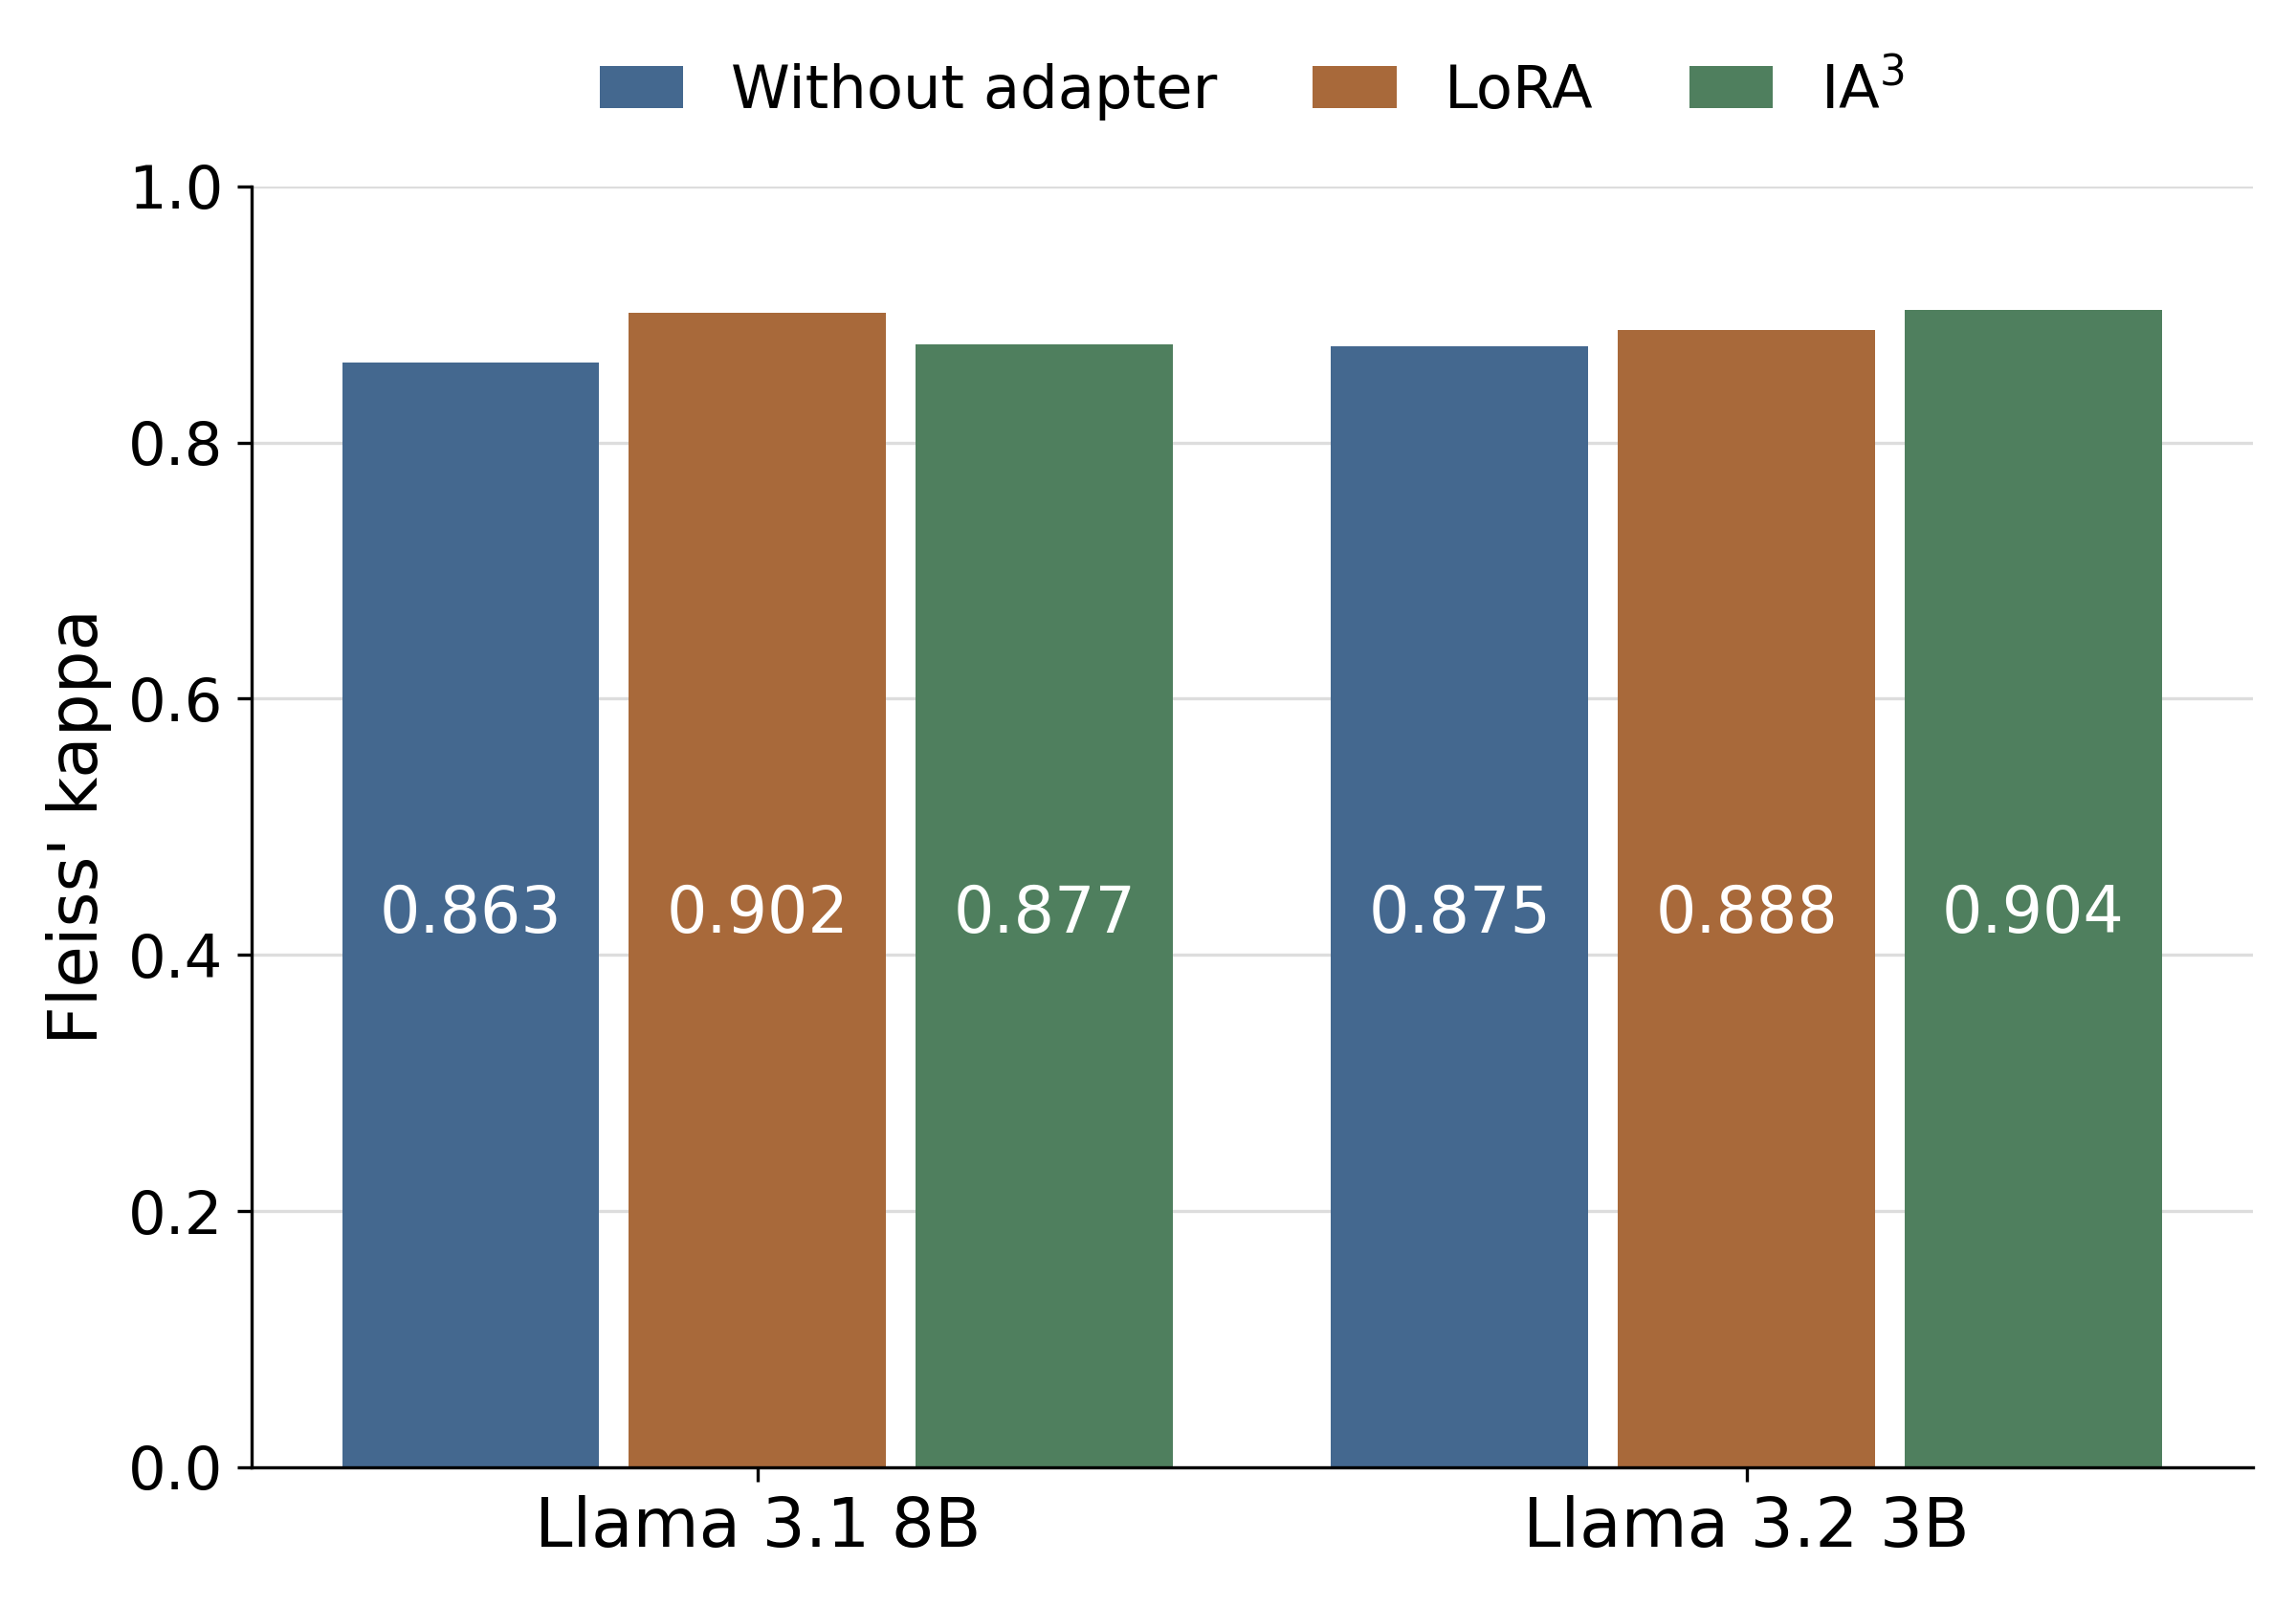
\includegraphics[width=12 cm]{figures/fig_kappa.png}
\caption{Fleiss' kappa for the six configurations.}\label{fig:kappa}
\end{figure}

Figure~\ref{fig:kappa} shows the same kappa values grouped by foundation model. The highest kappa was reached by Llama 3.2 3B + IA$^3$ (0.904), followed closely by Llama 3.1 8B + LoRA (0.902), and the lowest by Llama 3.1 8B without an adapter (0.863). The differences between the configurations are small. The confidence intervals are given in Table~\ref{tab:kappa}, and the paired comparisons in Section~\ref{sec:comparison} are used to test the differences between configurations, because they take into account that every configuration was rated on the same queries.

\subsection{Distribution of the Labels}\label{sec:labels}
Table~\ref{tab:labels} and Figure~\ref{fig:labels} show how often each label was used. These counts are descriptive. They are reported to show what the annotators decided and to explain the chance agreement in Table~\ref{tab:kappa}.

\begin{table}[H]
\caption{Number of ratings for each label and, in brackets, their share of the 4563 ratings given to each configuration (three annotators, 1521 queries), in percent.}\label{tab:labels}
\newcolumntype{C}{>{\centering\arraybackslash}X}
\begin{tabularx}{\textwidth}{lCCC}
\toprule
Configuration & Label 1 (agree) & Label 0 (neither) & Label $-1$ (disagree)\\
\midrule
Llama 3.1 8B & 2720 (59.6) & 389 (8.5) & 1454 (31.9)\\
Llama 3.1 8B + LoRA & 2862 (62.7) & 346 (7.6) & 1355 (29.7)\\
Llama 3.1 8B + IA$^3$ & 3544 (77.7) & 389 (8.5) & 630 (13.8)\\
Llama 3.2 3B & 2534 (55.5) & 441 (9.7) & 1588 (34.8)\\
Llama 3.2 3B + LoRA & 2449 (53.7) & 417 (9.1) & 1697 (37.2)\\
Llama 3.2 3B + IA$^3$ & 3414 (74.8) & 337 (7.4) & 812 (17.8)\\
\bottomrule
\end{tabularx}
\end{table}

Label 1 was given to 77.7\% of the ratings for Llama 3.1 8B + IA$^3$ and to 74.8\% for Llama 3.2 3B + IA$^3$. For the other four configurations, the share of label 1 was between 53.7\% and 62.7\%. Label $-1$ showed the opposite pattern: 13.8\% and 17.8\% for the two IA$^3$ configurations, and between 29.7\% and 37.2\% for the other four. Label 0 was used for between 7.4\% and 9.7\% of the ratings in every configuration. LoRA increased the share of label 1 for Llama 3.1 8B (62.7\% compared with 59.6\%) but not for Llama 3.2 3B (53.7\% compared with 55.5\%).

Figure~\ref{fig:labels} shows the same shares as stacked bars. The share of label 1 (agree) is the longest part of every bar, and the IA$^3$ bars have the smallest part for label $-1$ (disagree).

\begin{figure}[H]
\centering
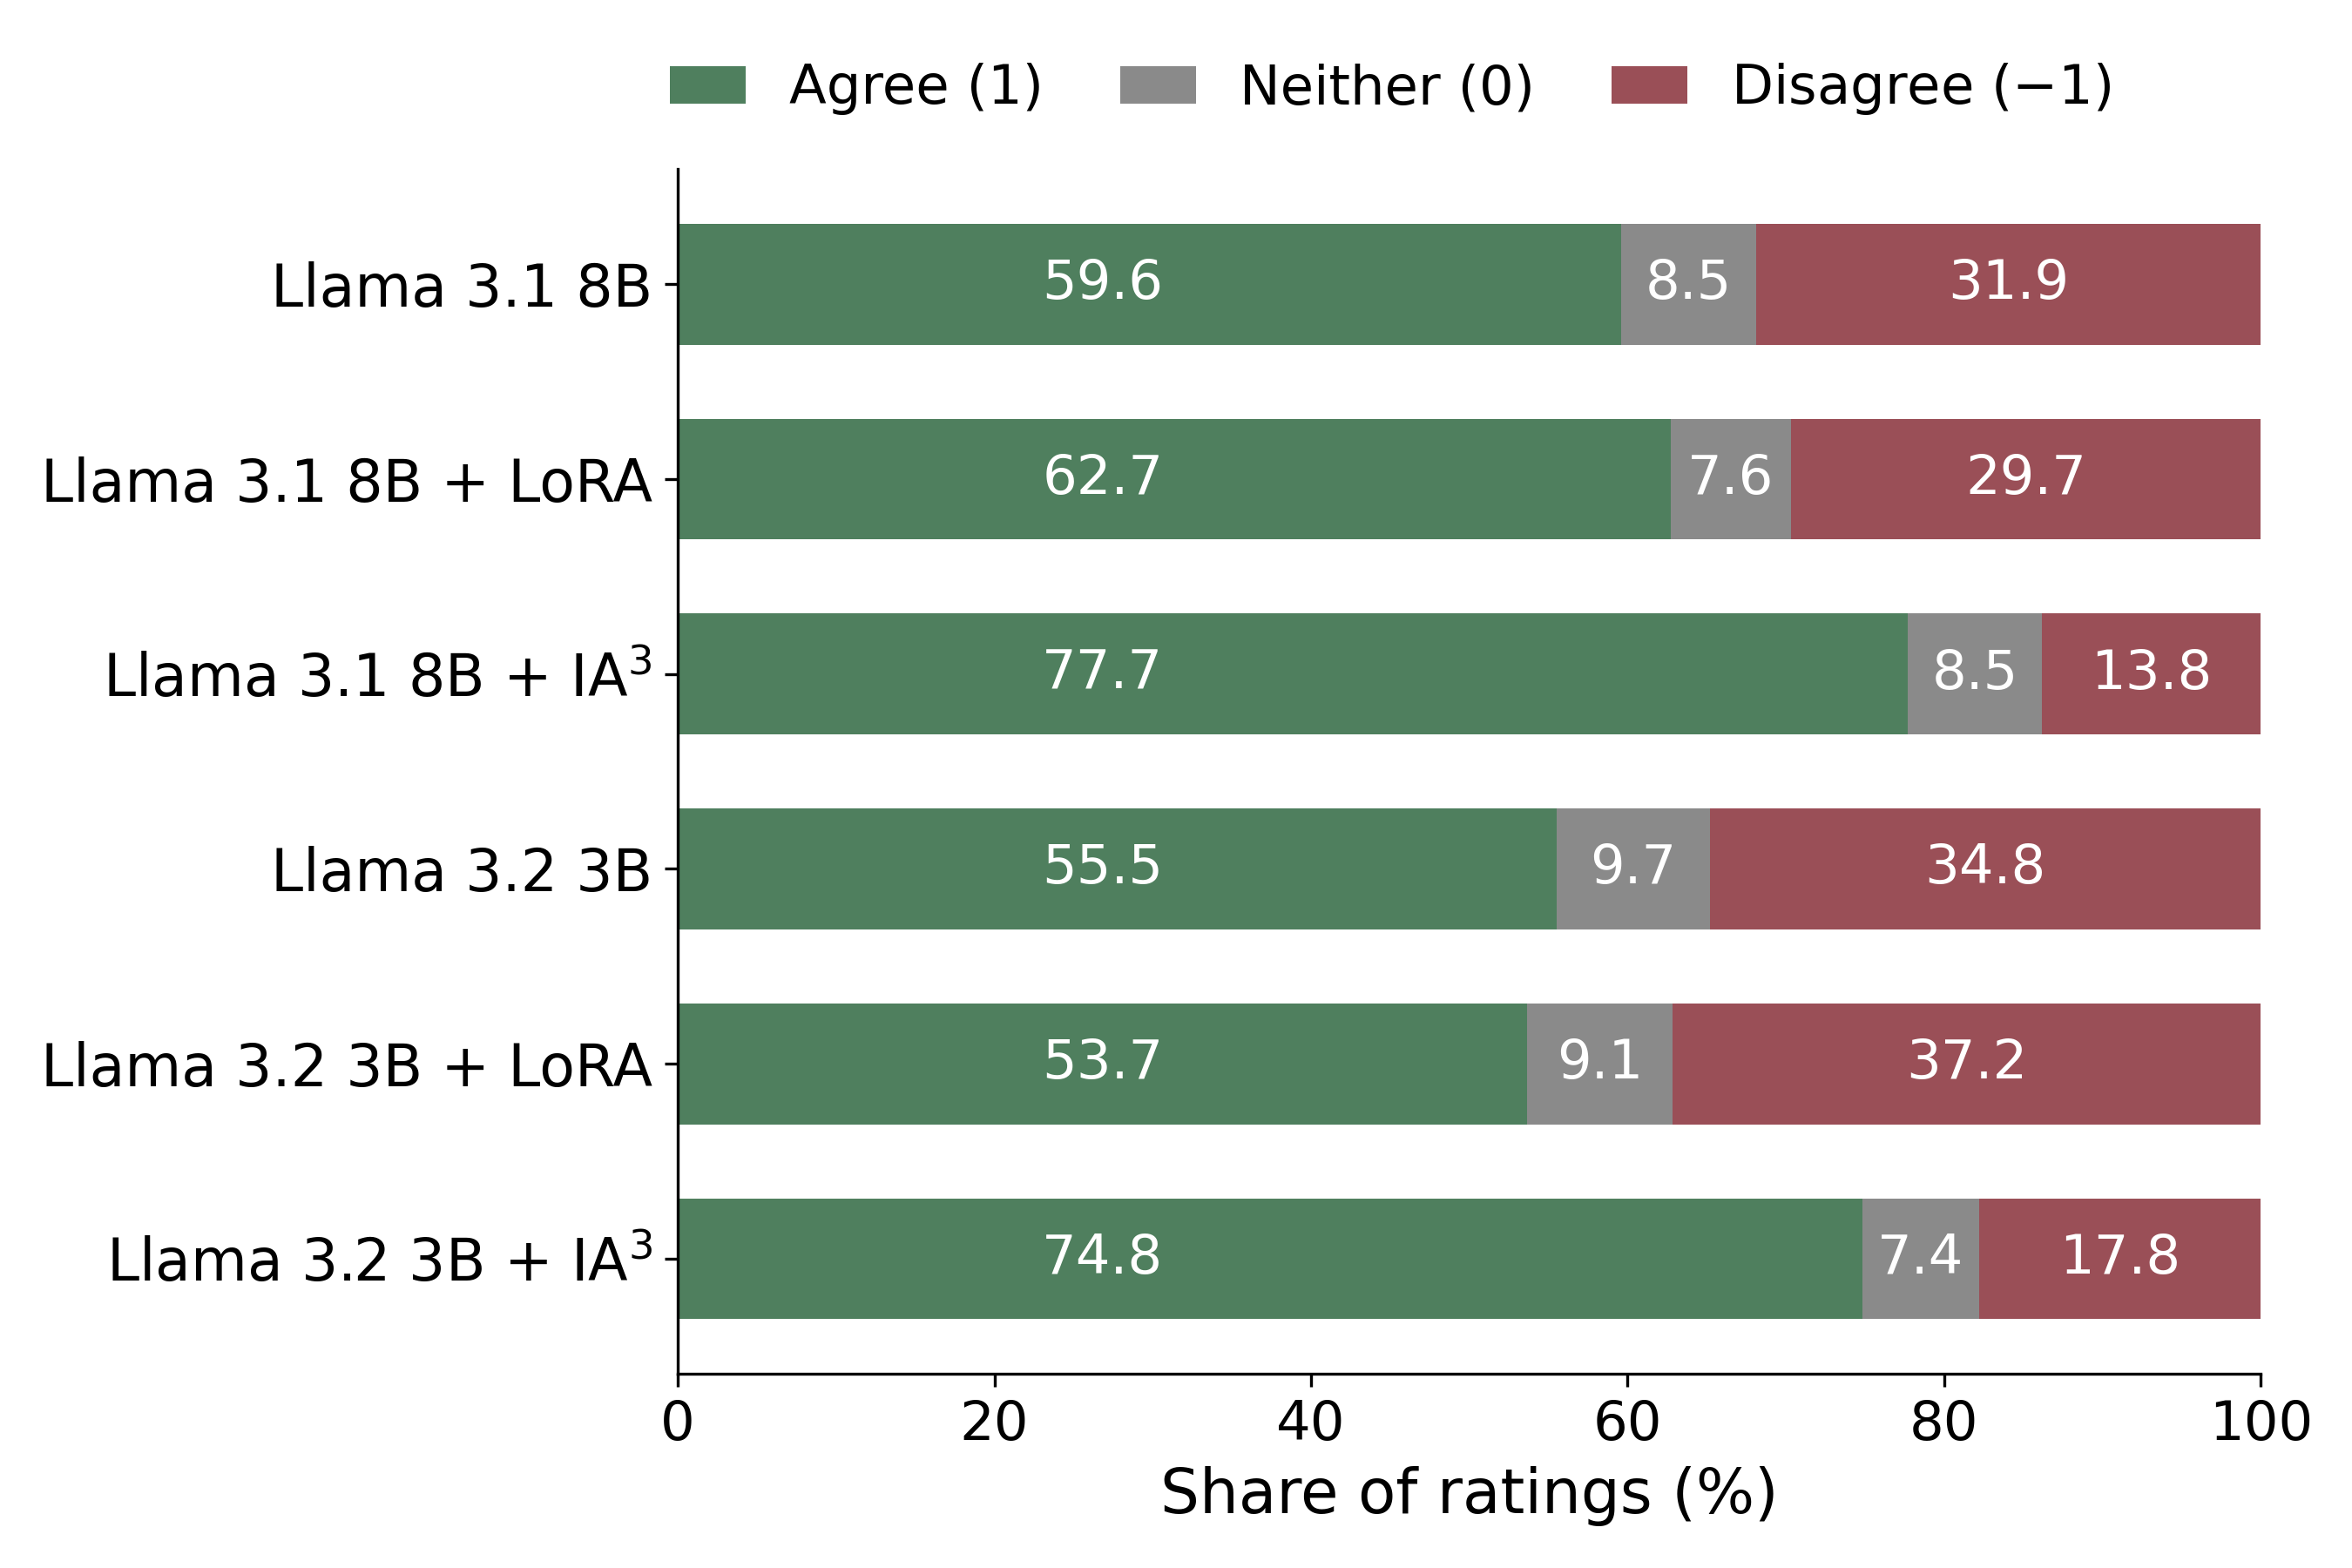
\includegraphics[width=12 cm]{figures/fig_labels.png}
\caption{Share of the ratings given to each label for the six configurations, in percent.}\label{fig:labels}
\end{figure}

These shares were not tested statistically, and Fleiss' kappa does not measure them. They show that the annotators agreed with the recommendations of the IA$^3$ configurations more often than with those of the other configurations. This may mean that the IA$^3$ recommendations matched the user profiles better, but this study did not test it.

\subsection{Comparison of the Adaptation Strategies}\label{sec:comparison}
Table~\ref{tab:comparisons} shows the nine planned comparisons. Each difference is the kappa of the configuration in the first column minus the kappa of the configuration in the second column.

\begin{table}[H]
\caption{Planned comparisons. Difference in Fleiss' kappa between the configuration in the first column and the configuration in the second column, its 95\% bootstrap confidence interval (CI) and the p-value adjusted with the Holm method for nine comparisons.}\label{tab:comparisons}
\newcolumntype{C}{>{\centering\arraybackslash}X}
\begin{tabularx}{\textwidth}{XXCCC}
\toprule
Configuration & Compared with & Difference & 95\% CI & Adjusted p\\
\midrule
Llama 3.1 8B + LoRA & Llama 3.1 8B & $+0.039$ & 0.014 to 0.064 & 0.015\\
Llama 3.1 8B + IA$^3$ & Llama 3.1 8B & $+0.014$ & $-0.016$ to 0.044 & 0.878\\
Llama 3.2 3B + LoRA & Llama 3.2 3B & $+0.013$ & $-0.011$ to 0.037 & 0.878\\
Llama 3.2 3B + IA$^3$ & Llama 3.2 3B & $+0.029$ & 0.002 to 0.055 & 0.262\\
Llama 3.1 8B + LoRA & Llama 3.1 8B + IA$^3$ & $+0.025$ & $-0.003$ to 0.053 & 0.458\\
Llama 3.2 3B + LoRA & Llama 3.2 3B + IA$^3$ & $-0.016$ & $-0.034$ to 0.003 & 0.458\\
Llama 3.1 8B & Llama 3.2 3B & $-0.012$ & $-0.037$ to 0.012 & 0.878\\
Llama 3.1 8B + LoRA & Llama 3.2 3B + LoRA & $+0.014$ & $-0.006$ to 0.033 & 0.717\\
Llama 3.1 8B + IA$^3$ & Llama 3.2 3B + IA$^3$ & $-0.027$ & $-0.056$ to 0.001 & 0.411\\
\bottomrule
\end{tabularx}
\end{table}

Hypothesis H2 expected that the models with adapters would be judged more consistently than the same models without adapters. All four adapter configurations had a higher kappa than the model without an adapter, with differences between $+0.013$ and $+0.039$. After the Holm correction, only the difference for LoRA on Llama 3.1 8B was statistically significant ($+0.039$, 95\% CI 0.014 to 0.064, adjusted p = 0.015). The difference for IA$^3$ on Llama 3.2 3B ($+0.029$) had an unadjusted p-value of 0.033 and an adjusted p-value of 0.262. H2 is therefore supported by the direction of all four differences, but by a statistically significant result for one comparison only.

Hypothesis H3 expected that LoRA would reach a higher agreement than IA$^3$. LoRA had a higher kappa on Llama 3.1 8B ($+0.025$) and a lower kappa on Llama 3.2 3B ($-0.016$). Neither difference was statistically significant (adjusted p = 0.458 for both). H3 is not supported.

Hypothesis H4 expected the same order of the strategies for both foundation models. The model without an adapter had the lowest kappa of its three configurations for both Llama 3.1 8B and Llama 3.2 3B. The order of LoRA and IA$^3$ was different for the two models. The same configuration did not differ significantly between the two foundation models: the differences (Llama 3.1 8B minus Llama 3.2 3B) were $-0.012$ without an adapter, $+0.014$ with LoRA and $-0.027$ with IA$^3$, with adjusted p-values between 0.411 and 0.878. The difference between the LoRA and IA$^3$ results was 0.041 larger for Llama 3.1 8B than for Llama 3.2 3B (95\% CI 0.008 to 0.074). This comparison was not one of the nine planned comparisons and was not adjusted. H4 is therefore supported for the position of the model without an adapter, but not for the order of the two adapters.

\subsection{Discussion}
The annotators reached almost perfect agreement for all six configurations. The test set contained only queries for which the annotators had not all marked the initial response with 1 during the ground truth annotation. Even so, the observed agreement for the recommendations of the six configurations was between 0.926 and 0.961. The annotators did not know which configuration produced each recommendation, so the agreement does not depend on knowledge of the model.

The differences in kappa between configurations were small, at most 0.041. No adapter configuration had a lower kappa than the same model without an adapter. Using LoRA or IA$^3$ therefore did not make the recommendations harder to judge consistently. The only difference that remained statistically significant after correction was LoRA on Llama 3.1 8B. There was no consistent difference between LoRA and IA$^3$, because the better adapter was not the same for the two foundation models. The same configuration also did not differ significantly between Llama 3.1 8B and Llama 3.2 3B.

The results for the IA$^3$ configurations show that kappa should be read together with the label distribution. These configurations received label 1 more often, which raised the chance agreement and lowered kappa relative to the observed agreement. Kappa measures how consistently the annotators judged the recommendations. It does not measure how accurate the recommendations are, so a higher kappa for one configuration does not show that its recommendations are better. The label shares in Table~\ref{tab:labels} point towards the IA$^3$ configurations as the ones whose recommendations the annotators accepted most often. A dedicated test of the label shares is needed to confirm this.

Some limits apply to these results. The recommendations are for one city, Pula, and were rated by three annotators. The test set contains only the queries that were difficult during annotation, and the label shares were not tested statistically. These and other limits are discussed in Section~\ref{sec:limitations}.

%%%%%%%%%%%%%%%%%%%%%%%%%%%%%%%%%%%%%%%%%%
\section{Limitations and Future Work}\label{sec:limitations}


%%%%%%%%%%%%%%%%%%%%%%%%%%%%%%%%%%%%%%%%%%
\section{Conclusions}

This section is not mandatory, but can be added to the manuscript if the discussion is unusually long or complex.

%%%%%%%%%%%%%%%%%%%%%%%%%%%%%%%%%%%%%%%%%%
\vspace{6pt} 

%%%%%%%%%%%%%%%%%%%%%%%%%%%%%%%%%%%%%%%%%%
%% optional
%\supplementary{The following supporting information can be downloaded at:  \linksupplementary{s1}, Figure S1: title; Table S1: title; Video S1: title.}

% Only for journal Methods and Protocols:
% If you wish to submit a video article, please do so with any other supplementary material.
% \supplementary{The following supporting information can be downloaded at: \linksupplementary{s1}, Figure S1: title; Table S1: title; Video S1: title. A supporting video article is available at doi: link.}

% Only used for preprtints:
% \supplementary{The following supporting information can be downloaded at the website of this paper posted on \href{https://www.preprints.org/}{Preprints.org}.}

% Only for journal Hardware:
% If you wish to submit a video article, please do so with any other supplementary material.
% \supplementary{The following supporting information can be downloaded at: \linksupplementary{s1}, Figure S1: title; Table S1: title; Video S1: title.\vspace{6pt}\\
%\begin{tabularx}{\textwidth}{lll}
%\toprule
%\textbf{Name} & \textbf{Type} & \textbf{Description} \\
%\midrule
%S1 & Python script (.py) & Script of python source code used in XX \\
%S2 & Text (.txt) & Script of modelling code used to make Figure X \\
%S3 & Text (.txt) & Raw data from experiment X \\
%S4 & Video (.mp4) & Video demonstrating the hardware in use \\
%... & ... & ... \\
%\bottomrule
%\end{tabularx}
%}

%%%%%%%%%%%%%%%%%%%%%%%%%%%%%%%%%%%%%%%%%%
\authorcontributions{Conceptualization, R.K.,  L.S. and S.B.Š.; methodology, L.S.; software, R.K.; validation, I.L. and S.B.Š.; formal analysis, R.K.; investigation, R.K. and L.S.; resources, R.K.; data curation, R.K. and L.S.; writing—original draft preparation, R.K. and L.S.; writing—review and editing, S.B.Š. and I.L.; visualization, R.K.; supervision, S.B.Š. and I.L.; project administration, S.B.Š. and I.L.; funding acquisition, I.L. All authors have read and agreed to the published version of the manuscript.}

\funding{This work was (partially) supported by the EC Digital Europe Programme EDIH Adria 2.0 (101256325); SPIN projects IP.1.1.03.0120, IP.1.1.03.0158 and IP.1.1.03.0039; and NextGenerationEU University grants: uniri-iz-25-6, uniri-iz-25-220, IIP\_010144, IIP\_010136}

% \institutionalreview{In this section, you should add the Institutional Review Board Statement and approval number, if relevant to your study. You might choose to exclude this statement if the study did not require ethical approval. Please note that the Editorial Office might ask you for further information. Please add “The study was conducted in accordance with the Declaration of Helsinki, and approved by the Institutional Review Board (or Ethics Committee) of NAME OF INSTITUTE (protocol code XXX and date of approval).” for studies involving humans. OR “The animal study protocol was approved by the Institutional Review Board (or Ethics Committee) of NAME OF INSTITUTE (protocol code XXX and date of approval).” for studies involving animals. OR “Ethical review and approval were waived for this study due to REASON (please provide a detailed justification).” OR “Not applicable” for studies not involving humans or animals.}

% \informedconsent{Any research article describing a study involving humans should contain this statement. Please add ``Informed consent was obtained from all subjects involved in the study.'' OR ``Patient consent was waived due to REASON (please provide a detailed justification).'' OR ``Not applicable'' for studies not involving humans. You might also choose to exclude this statement if the study did not involve humans.

% Written informed consent for publication must be obtained from participating patients who can be identified (including by the patients themselves). Please state ``Written informed consent has been obtained from the patient(s) to publish this paper'' if applicable.}

\dataavailability{The original data presented in this study are openly available in a public repository at \url{https://www.mdpi.com/ethics}.} 

%\durcstatement{Current research is limited to the [please insert a specific academic field, e.g., XXX], which is beneficial [share benefits and/or primary use] and does not pose a threat to public health or national security. Authors acknowledge the dual-use potential of the research involving xxx and confirm that all necessary precautions have been taken to prevent potential misuse. As an ethical responsibility, authors strictly adhere to relevant national and international laws about DURC. Authors advocate for responsible deployment, ethical considerations, regulatory compliance, and transparent reporting to mitigate misuse risks and foster beneficial outcomes.}

% Only for journal Nursing Reports
%\publicinvolvement{Please describe how the public (patients, consumers, carers) were involved in the research. Consider reporting against the GRIPP2 (Guidance for Reporting Involvement of Patients and the Public) checklist. If the public were not involved in any aspect of the research add: ``No public involvement in any aspect of this research''.}
%
%% Only for journal Nursing Reports
%\guidelinesstandards{Please add a statement indicating which reporting guideline was used when drafting the report. For example, ``This manuscript was drafted against the XXX (the full name of reporting guidelines and citation) for XXX (type of research) research''. A complete list of reporting guidelines can be accessed via the equator network: \url{https://www.equator-network.org/}.}
%
%% Only for journal Nursing Reports
%\useofartificialintelligence{Please describe in detail any and all uses of artificial intelligence (AI) or AI-assisted tools used in the preparation of the manuscript. This may include, but is not limited to, language translation, language editing and grammar, or generating text. Alternatively, please state that “AI or AI-assisted tools were not used in drafting any aspect of this manuscript”.}

\acknowledgments{This research was performed using the Advanced computing service provided by University of Zagreb University Computing Centre - SRCE.}

\conflictsofinterest{The authors declare no conflicts of interest.} 

%%%%%%%%%%%%%%%%%%%%%%%%%%%%%%%%%%%%%%%%%%
%% Optional

%% Only for journal Encyclopedia
%\entrylink{The Link to this entry published on the encyclopedia platform.}

\abbreviations{Abbreviations}{
The following abbreviations are used in this manuscript:
\\

\noindent 
\begin{tabular}{@{}ll}
LLMs & Large Language Models\\
NLP & Natural Language Processing\\
PEFT & Parameter-Efficient Fine-Tuning\\
LoRA & Low-Rank Adaptation\\
IA$^3$ & Infused Adapter by Inhibiting and Amplifying Inner Activations\\
ICL & In-Context Learning\\
JSON & JavaScript Object Notation\\
SFT & Supervised Fine-Tuning\\
GPU & Graphics Processing Unit\\
DDP & Distributed Data Parallel\\
MLP & Multi-Layer Perceptron\\
bf16 & BFloat16 Precision Format\\
tf32 & TensorFloat-32\\
\end{tabular}
}

%%%%%%%%%%%%%%%%%%%%%%%%%%%%%%%%%%%%%%%%%%
%\isPreprints{}{% This command is only used for ``preprints''.
\begin{adjustwidth}{-\extralength}{0cm}
%} % If the paper is ``preprints'', please uncomment this parenthesis.
%\printendnotes[custom] % Un-comment to print a list of endnotes

\reftitle{References}

% Please provide either the correct journal abbreviation (e.g. according to the “List of Title Word Abbreviations” http://www.issn.org/services/online-services/access-to-the-ltwa/) or the full name of the journal.
% Citations and References in Supplementary files are permitted provided that they also appear in the reference list here. 

%=====================================
% References, variant A: external bibliography
%=====================================
\bibliography{references}

% If authors have biography, please use the format below
%\section*{Short Biography of Authors}
%\bio
%{\raisebox{-0.35cm}{\includegraphics[width=3.5cm,height=5.3cm,clip,keepaspectratio]{Definitions/author1.pdf}}}
%{\textbf{Firstname Lastname} Biography of first author}
%
%\bio
%{\raisebox{-0.35cm}{\includegraphics[width=3.5cm,height=5.3cm,clip,keepaspectratio]{Definitions/author2.jpg}}}
%{\textbf{Firstname Lastname} Biography of second author}

% For the MDPI journals use author-date citation, please follow the formatting guidelines on http://www.mdpi.com/authors/references
% To cite two works by the same author: \citeauthor{ref-journal-1a} (\citeyear{ref-journal-1a}, \citeyear{ref-journal-1b}). This produces: Whittaker (1967, 1975)
% To cite two works by the same author with specific pages: \citeauthor{ref-journal-3a} (\citeyear{ref-journal-3a}, p. 328; \citeyear{ref-journal-3b}, p.475). This produces: Wong (1999, p. 328; 2000, p. 475)

%%%%%%%%%%%%%%%%%%%%%%%%%%%%%%%%%%%%%%%%%%
%% for journal Sci
%\reviewreports{\\
%Reviewer 1 comments and authors’ response\\
%Reviewer 2 comments and authors’ response\\
%Reviewer 3 comments and authors’ response
%}
%%%%%%%%%%%%%%%%%%%%%%%%%%%%%%%%%%%%%%%%%%
\PublishersNote{}
%\isPreprints{}{% This command is only used for ``preprints''.
\end{adjustwidth}
%} % If the paper is ``preprints'', please uncomment this parenthesis.
\end{document}